\section{Section 3.3}

\subsection{Murphy - 3.20}
\subsubsection{Part(a)}
If we take the distribution of the binary vectors separately, then we are forced to assign a probability distribution over all the $2^D$ vectors for a particular $y = c$
Since there are only finitely many , we can use a categorical for every class over all the vectors
\begin{equation}
    p(x|y = c) =  \textbf{Cat}(x | \vb{\theta_c}) \ \ \ \theta_c \in \mathbb{R}^{2^D}  \ \ \ \sum(\vb{\theta_c}) = 1
\end{equation}
Number of parameters = $(2^D - 1) \times C$
\subsubsection{Part(b)}
If the sample size is large, the case with large number of parameters (non Naive- modelling) will be able to perform better than the Naive classifier, because the Non-Naive Model is a superset of the Naive model, and therefore the Non-Naive model will perform better on training of parameters through a sufficient number of examples.

\subsubsection{Part (c)}
If the number of examples are insufficient, it will be very difficult to train the large number of parameters of the Non-Naive case. However the Naive case has lesser parameters and hence the model will be able to learn better with lesser number of samples to work with.

\subsubsection{Part (d), (e)}


\subsection{Murphy - 3.22}
We only need to take the fraction of the examples where that particular word in the vocabular occurs  (since this is a Bernoulli Model, these will be the likelihood estimates)
\begin{gather}
    \text{Total examples} = 3 + 4 = 7\\
    \theta_{non-spam} = 4/7\\
    \theta_{spam} = 3/7\\
    \theta_{secret | spam} = 2/3\\
    \theta_{dollar| spam} = 1/3\\
    \theta_{sports | non-spam} = 2/4\\
    \theta_{secret| non-spam} = 1/4
\end{gather}
\subsection{Murphy 4.18}
 $$\theta = 0.5, 0.5 , 0.5 \ \ \ \ \ \ \ \mu  = \mu_c , \sigma  = \sigma_c   \ \ \ \forall c $$
See that all the classes model the same Normal and Bernoulli Distributions!, the naive baye's classifier ( which assumes conditional independence) will not be actually say anything more about the conditional $p(y|x)$ than what p(y) would say(the prior is the only way to judge an example, 
Since a single value of x are all equally weighted by the class conditionals.)

\begin{gather}
    p(y_i|x) =  \frac{p(x_1|y_i)p(y_i)}{\sum p(x_1|y_j)p(y_j)} = \frac{p(y_i)}{\sum(p(y_i))} = p(y_i)
\end{gather}

So for all of them the answer will be
\begin{gather}
    p(y |x_1 = 0) = p(y | x_2 = 0) = p(y | x_1,x_2 = 0) =  \vb{\pi} = [0.5, 0.25, 0.25]
\end{gather}
\subsection{Murphy 4.19}
The expression will not boil down much, the determinants of the covariances will be related though, this will simplify the expression (Uniform prior has been assumed)

\begin{gather*}
    p(y = 1| x)  = \frac{p(y = 1, x)}{\sum p(x = i | y)p(y)}
    \\
    p(y = 1| x)  = \frac{1/|\Sigma_1|^{1/2}}{1/|\Sigma_1|^{1/2}\textbf{Gau}(x|y=1) + 1/|\Sigma_0|^{1/2}\textbf{Gau}(x|y = 0) }
    \\
    |\Sigma_1| = k^d |\Sigma_0 | \ \ \ \ \& \ \ \ \  \Sigma_1^{-1} = \frac{\Sigma_0^{-1} }{k}
    \\
     f_c(x) = -\frac{1}{2}(x - \mu_c)^T\Sigma_c(x - \mu_c)
     \\
    p(y = 1 | x) = \frac{1}{1 + k^{d/2}\exp(f_0(x) - f_1(x))}
    \\
    p(y = 1 | x) = \frac{1}{1 + \exp(f_0(x) - f_1(x) + d/2 \ln(k))}
    \\
     p(y = 1 | x) = \frac{1}{1 + \exp(f_0(x) - f_1(x) + d/2 \ln(k))}
     \\
     p(y = 1 | x) = \frac{1}{1 + \exp(-\frac{1}{2}( x^TAx + bx + C))} \\
     \\
     A = \frac{k - 1}{2k} (\Sigma_0^{-1})
     \\
     b = \frac{2}{k}(k\mu_0^T  - \mu_1^T)(\Sigma_0)^{-1}
\end{gather*}
Geometric interpretation
If the value of k increases the probability of lying in the 1st class decreases , (more spread out, so inorder to  compensate for this the decision surface will now move closer to the mean of the class - 1 distribution.

Decision surface:- I believe the decision surface will be some sort of hyperbolic surface, the Mahalanobis distances when subtracted yield a  constant.

\begin{equation}
    (x - \mu_0)^T\Sigma_0^{-1}(x - \mu_1)^T - \frac{1}{k}(x - \mu_1)^T\Sigma_0^{-1}(x - \mu_1)^T =\frac{d}{2}ln(k)
\end{equation}

\subsection{Problem 4.21}
The decision region is just the equality of the probabilities of the class conditionals ( since the priors are the same)
on solving the equation we get two values for x 
\begin{gather}
    \frac{(x - \mu_2)^2}{2 \sigma_2^2} - \frac{(x - \mu_1)^2}{2 \sigma_1^2} = \ln(\frac{\sigma_1}{\sigma_2}) \\
    \text{On solving we get } \ x = -3.717 , 3.717
    \\ 
    \text{Staying in between the roots gives negative inequality  } 
    \\R_1 = \ x \in [-3.717, 3.717] 
    \\
    \sigma_2 = 1 , x \le 0.5
\end{gather}
To see the code please visit \cite{CS3390}
\begin{figure}[!h]
    \centering
    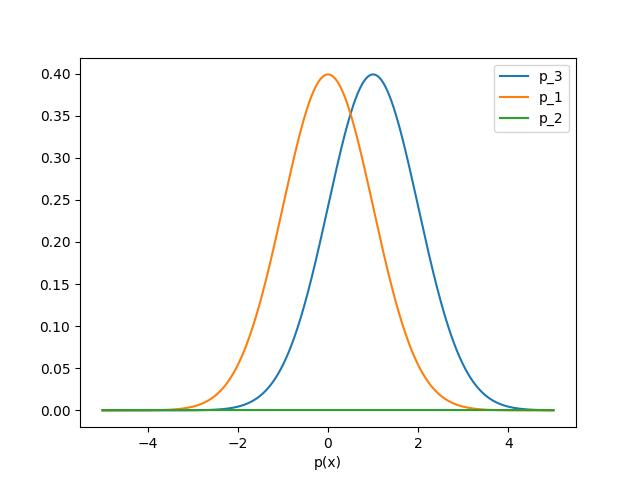
\includegraphics[scale = 0.5]{Murphy-4.21.jpg}
    \caption{Plots of the class conditionals}
\end{figure}

\subsection{Problem 4.22}
We can write our code for a bayes classiifer for these points, see \cite{CS3390}. Please note that the 
priors are uniform , so they play no role in calculating the denisties.
we need only calculate the values of the class conditionals and take the class that assigns maximum probability,
here are the density vectors for both the examples
\begin{gather}
    x_1 = [0.5, 0.5] \ p_1, p_2, p_3  = \    [0.15908049 , 0.16001875,  0.03022364] \\
    \\
    \therefore   Class(x_1) = 2
    \\
    x_2 = [-0.5, 0.5] \ p_1, p_2, p_3 = \ [0.04983036 , 0.04983036,  0.13545295]
    \\
    \therefore Class(x_2) = 1,2
\end{gather}
\subsection{Problem 4.23}
For the code please see \cite{CS3390}.
Please note that the prior is uniform, so it plays no role in finding the maximum score
The male is assumed to be class 0 
\begin{gather}
    p(y = m | x) = \frac{p(x = m | y)p(y)}{\sum_c ( p ( x = c | y  = c)p(y =c))}
    \\
    \mu_0 , \mu_1 = 72.333, 65.0
    \\
    \sigma_0 , \sigma_1  = 4.988, 3.559
    \\
    \pi_c = 0.5
    \\
    p(y  = m | x = 72) = 0.8312
\end{gather}

